% Chapter 5

\chapter{Implementation and Results} % Main chapter title

\label{Chapter5}

%----------------------------------------------------------------------------------------

\section{Introduction to the Optimization Engine}

The transition from data ingestion to the core solver introduces a highly constrained NP-hard optimization problem. The IIITA Timetabling System models this challenge mathematically, solving it via client-side heuristics. Rather than relying on traditional deterministic approaches which fail to scale, the system employs an evolutionary search mechanism. The engine processes high-dimensional inputs---comprising student cohorts, faculty assignments, and spatial capacities---and systematically navigates a vast, discontinuous search space to identify a globally optimal, conflict-free schedule.

\begin{figure}[htbp]
\centering
\resizebox{\textwidth}{!}{%
\begin{tikzpicture}[
    actor/.style={rectangle, draw, fill=blue!10, text width=1.8cm, align=center, font=\sffamily\scriptsize, minimum height=0.7cm, rounded corners=2pt},
    lifeline/.style={dashed, gray},
    msg/.style={->, >=stealth, thick, font=\sffamily\tiny},
    rmsg/.style={->, >=stealth, thick, dashed, font=\sffamily\tiny},
    activation/.style={fill=blue!8, draw, minimum width=0.3cm},
    note/.style={rectangle, draw, fill=yellow!10, text width=3cm, align=left, font=\sffamily\tiny, rounded corners}
]

% Actors
\node[actor] (admin) at (0,0) {\textbf{Admin}};
\node[actor] (gen) at (3.5,0) {\textbf{Generator\\View}};
\node[actor] (db) at (7,0) {\textbf{Supabase\\DB}};
\node[actor] (prep) at (10.5,0) {\textbf{dataPrep}};
\node[actor] (solver) at (14,0) {\textbf{Solver\\Engine}};

% Lifelines
\foreach \x in {admin, gen, db, prep, solver} {
    \draw[lifeline] (\x.south) -- ++(0,-14);
}

% Messages
\draw[msg] (0,-1.2) -- node[above] {1. Select Cluster} (3.5,-1.2);
\draw[msg] (3.5,-1.8) -- node[above] {2. Fetch subjects, groups} (7,-1.8);
\draw[rmsg] (7,-2.4) -- node[above] {3. Return cluster data} (3.5,-2.4);

\draw[msg] (0,-3.2) -- node[above] {4. Map rooms, assign profs} (3.5,-3.2);

\draw[msg] (0,-4.0) -- node[above] {5. Configure seed \& locks} (3.5,-4.0);
\draw[msg] (3.5,-4.6) -- node[above] {6. Fetch locked slots} (7,-4.6);
\draw[rmsg] (7,-5.2) -- node[above] {7. Return locked sessions} (3.5,-5.2);

\draw[msg] (0,-6.0) -- node[above] {8. Click ``Generate''} (3.5,-6.0);
\draw[msg] (3.5,-6.6) -- node[above] {9. prepareSolverInput()} (10.5,-6.6);
\draw[rmsg] (10.5,-7.2) -- node[above] {10. SolverInput bundle} (3.5,-7.2);

\draw[msg] (3.5,-7.8) -- node[above] {11. runSolver(input)} (14,-7.8);

% Solver loop
\draw[msg] (14,-8.6) -- node[above] {12. onProgress()} (3.5,-8.6);
\node[note, right=0.3cm of solver, yshift=-9cm] (loop) {Repeats every\\reportInterval\\generations};
\draw[rmsg] (14,-9.4) -- node[above] {13. onProgress()} (3.5,-9.4);

\draw[rmsg] (14,-10.4) -- node[above] {14. SolverResult} (3.5,-10.4);

\draw[msg] (0,-11.2) -- node[above] {15. Click ``Save''} (3.5,-11.2);
\draw[msg] (3.5,-11.8) -- node[above] {16. INSERT timetable + slots} (7,-11.8);
\draw[rmsg] (7,-12.4) -- node[above] {17. Confirm saved} (3.5,-12.4);
\draw[rmsg] (3.5,-13.0) -- node[above] {18. Navigate to EditorView} (0,-13.0);

\end{tikzpicture}
}%
\caption{Sequence Diagram: End-to-End Intelligent Generator Workflow}
\label{fig:generator_sequence}
\end{figure}

\section{Mathematical Representation of the Schedule}

To facilitate computational optimization, the schedule is encoded into a specific data structure known as a \textit{Chromosome}. The solver models a complete timetable $S$ as an ordered array of \textit{genes}. Each gene $g_i \in S$ encodes the precise scheduling decision for the $i$-th class session, mapping it to a spatial and temporal coordinate. 

Formally, a gene is defined as a tuple:
\begin{equation}
    g_i = (d_i, t_i, r_i)
\end{equation}
where:
\begin{itemize}
    \item $d_i \in \{1, 2, 3, 4, 5\}$ represents the day of the week (Monday through Friday).
    \item $t_i \in \{1, 2, \dots, 8\}$ represents the discrete start time slot (each slot corresponding to one hour, from 08:50 to 18:30).
    \item $r_i \in \mathcal{R}$ is the index into the array of available physical rooms.
\end{itemize}

Each gene is invariably linked to an immutable \texttt{ClassSession} object that contains the session's metadata: the specific subject identifier, the student group $G_i$, the assigned professor $p_i$, the duration $D_i$, and the specific slot type (Lecture, Tutorial, or Practical).

\section{Mathematical Formulation of Constraints}

The optimization objective is governed by a composite fitness function that evaluates both the feasibility and the quality of the candidate solution $S$.

\subsection{Hard Constraints (The Feasibility Space)}

Hard constraints define the boundary of feasible solutions. A schedule is strictly invalid if any hard constraint is violated. For two distinct sessions $i$ and $j$, we define the temporal overlap condition as:
\begin{equation}
    \text{overlap}(t_i, t_j) = \begin{cases} 
      1 & \text{if } \max(t_i, t_j) \le \min(t_i + D_i - 1, t_j + D_j - 1) \\
      0 & \text{otherwise}
   \end{cases}
\end{equation}

The engine enforces the following critical hard penalties:
\begin{itemize}
    \item \textbf{Professor Overlap Penalty:} A professor $p$ cannot be physically present in two different locations at time $t$. 
    \begin{equation}
        \sum_{i \neq j} \mathbb{I}(p_i = p_j \land d_i = d_j \land \text{overlap}(t_i, t_j)) = 0
    \end{equation}

    \item \textbf{Student Group Overlap Penalty:} A specific student cohort $G$ cannot attend two distinct subjects simultaneously. (Concurrent sessions from the same synchronized elective basket are mathematically exempted).
    \begin{equation}
        \sum_{i \neq j} \mathbb{I}(G_i = G_j \land d_i = d_j \land \text{overlap}(t_i, t_j) \land \neg \text{SameBasket}(i, j)) = 0
    \end{equation}

    \item \textbf{Room Clash Penalty:} A physical room $r$ can host at most one session at any given time.
    \begin{equation}
        \sum_{i \neq j} \mathbb{I}(r_i = r_j \land d_i = d_j \land \text{overlap}(t_i, t_j)) = 0
    \end{equation}

    \item \textbf{Lunch Boundary Enforcement:} Sessions cannot cross the designated lunch break ($B_{lunch}$ from 13:00 to 14:30, bounded between slot 4 and 5). 
    \begin{equation}
        \forall i \in S, \quad [t_i, t_i + D_i - 1] \cap B_{lunch} = \emptyset
    \end{equation}

    \item \textbf{L-T-P ``Chunking'' (The 2+1 Rule):} For core courses with $L \ge 2$ credits, the algorithm mathematically forces the contact hours into a contiguous 2-hour block and subsequent 1-hour blocks, distributed across distinct days. Let $\mathcal{L}_c$ be the set of lecture sessions for subject $c$:
    \begin{equation}
        \exists! k \in \mathcal{L}_c : D_k = 2 \quad \text{and} \quad \forall j \in \mathcal{L}_c \setminus \{k\}, D_j = 1
    \end{equation}
    \begin{equation}
        \forall i, j \in \mathcal{L}_c, \ i \neq j \implies d_i \neq d_j
    \end{equation}
\end{itemize}

\begin{table}[htbp]
\centering
\caption{Hard Constraints Enforced by the Solver}
\label{tab:hard_constraints}
\renewcommand{\arraystretch}{1.4}
\begin{tabularx}{\textwidth}{@{} c l X @{}}
\toprule
\textbf{\#} & \textbf{Constraint Name} & \textbf{Description} \\
\midrule
1 & Time Boundary & A session must not extend beyond slot 8 (18:30). \\
2 & Break/Lunch Crossing & A multi-slot session must not span across a break boundary (slots 2$\to$3 or 4$\to$5). \\
3 & Room Non-Overlap & At most one session may occupy a given room at any (day, slot). \\
4 & Professor Non-Overlap & A professor can teach at most one session at any given slot. No elective exemption. \\
5 & Group Non-Overlap & A student group can attend at most one session per slot. Elective--elective pairs and same-basket pairs are exempt. \\
6 & Elective Basket Sync & Synced baskets (HSMC, MDM) must share the same (day, slot). No two different baskets may share a slot (global anti-clash). \\
7 & Lab Room & Practical sessions must be assigned to rooms with type ``Lab''. \\
8 & WMC-Section Overlap & A whole-batch (WMC) session cannot occupy the same slot as any section-level session. \\
9 & Home Room & Core lectures and tutorials must be placed in their assigned home room. \\
10 & 2+1 Lecture Format & The double-lecture block and single-lectures for the same subject+group must be on different days. \\
\bottomrule
\end{tabularx}
\end{table}

\subsection{Soft Constraints (The Quality Space)}

Once the solution space is feasible, the engine optimizes for schedule quality by minimizing soft penalties.

\begin{itemize}
    \item \textbf{Minimizing Student Gaps:} The engine minimizes idle slots between a cohort's first and last class on any given day. Let $\mathcal{T}_{g,d}$ be the set of all active time slots for student group $g$ on day $d$. The gap penalty $G(S)$ is:
    \begin{equation}
        G(S) = \sum_{g} \sum_{d} \left( (\max(\mathcal{T}_{g,d}) - \min(\mathcal{T}_{g,d}) + 1) - |\mathcal{T}_{g,d}| \right)
    \end{equation}

    \item \textbf{Room Capacity Optimization:} The system matches class enrollment $c_i$ to room capacity $K_{r_i}$. Let the utilization ratio be $u_i = c_i / K_{r_i}$. Given optimal thresholds $\alpha = 0.6$ and $\beta = 1.2$, the room utilization penalty $R(S)$ is formulated as:
    \begin{equation}
        R(S) = \sum_{i} \left( \max(0, \alpha - u_i) + \max(0, u_i - \beta) \right)
    \end{equation}
\end{itemize}

\section{The (1+1) Evolution Strategy Solver}

The optimization engine is powered by a (1+1) Evolution Strategy (ES) algorithm. It relies on iterative stochastic perturbations and adaptive mutation rates to navigate the constrained schedule space.

\subsection{Strict Elitism}

The algorithm employs a strictly elitist selection mechanism. In each generation, a parent solution $S_{parent}$ undergoes mutation to produce a single offspring $S_{child}$. The offspring replaces the parent if and only if its total fitness score is less than or equal to the parent's score:
\begin{equation}
    S_{parent}^{(t+1)} = \begin{cases} 
      S_{child} & \text{if } f(S_{child}) \le f(S_{parent}^{(t)}) \\
      S_{parent}^{(t)} & \text{otherwise}
   \end{cases}
\end{equation}
This greediness guarantees that the solver never loses ground on hard constraint feasibility.

\subsection{Mutation Operators}

To generate $S_{child}$, the engine selects a subset of mutable sessions and applies highly stochastic operators:
\begin{itemize}
    \item \textbf{Gaussian Time Shifts:} The start time $t_i$ is perturbed using Gaussian noise scaled by variance $\sigma$:
    \begin{equation}
        t_i^{(new)} = t_i + \lfloor \mathcal{N}(0, \sigma^2) \rceil
    \end{equation}
    \item \textbf{Type-Aware Room Reassignments:} A session is moved to a randomly selected room $r_k \in \mathcal{R}$ that strictly matches its required architectural type (e.g., Lab vs. Lecture Hall).
    \item \textbf{Targeted Swaps:} Two sessions $i$ and $j$ of identical duration exchange their spatial-temporal coordinates, effectively jumping out of local minima without increasing the overall density.
\end{itemize}

\subsection{Adaptive Variance (The Brain)}

To dynamically balance global exploration and local exploitation, the solver implements Rechenberg's 1/5th Success Rule. The mutation strength $\sigma$ is adapted every $W = 50$ generations based on the success rate $p_s$ (the ratio of offspring that successfully improved or matched fitness).
\begin{equation}
    \sigma \leftarrow
    \begin{cases}
        \sigma \times 1.22 & \text{if } p_s > 0.20 \quad \text{(Search wider)} \\
        \sigma \times 0.82 & \text{if } p_s < 0.20 \quad \text{(Search finer)} \\
        \sigma & \text{otherwise}
    \end{cases}
\end{equation}

\subsection{Stagnation Recovery}

In highly dense optimization landscapes, the algorithm may converge to a deep local optimum (a plateau). The engine mathematically tracks this stagnation. If $S_{parent}$ fails to improve for 15,000 consecutive generations, a stagnation recovery protocol is triggered. The current candidate is discarded, and maximum entropy is injected by generating a completely new randomized initial timetable.

\begin{figure}[htbp]
\centering
\begin{tikzpicture}[
    node distance=1.1cm,
    start/.style={draw, circle, fill=black, minimum size=6pt, inner sep=0pt},
    stop/.style={draw, circle, fill=black, minimum size=6pt, inner sep=0pt, double, double distance=1.5pt},
    action/.style={draw, rectangle, fill=blue!8, rounded corners=3pt, text width=6cm, align=center, font=\sffamily\scriptsize, minimum height=0.6cm},
    decision/.style={draw, diamond, aspect=2.5, fill=orange!10, text width=1.8cm, align=center, font=\sffamily\scriptsize, inner sep=1pt},
    arrow/.style={draw, thick, ->, >=stealth, font=\sffamily\tiny}
]

\node[start] (s) {};
\node[action, below=of s] (init) {Generate Initial Solution\\(round-robin day, break-aware slot)};
\node[action, below=of init] (seed) {Apply Seed \& Pin Locked Genes};
\node[action, below=of seed] (mutate) {Mutate Parent $\to$ Offspring\\(3--8\% of mutable sessions)};
\node[action, below=of mutate] (eval) {Evaluate Offspring Fitness $f(S')$};
\node[decision, below=of eval] (accept) {$f(S') \leq f(S)$\,?};
\node[action, below left=1.2cm and 0.3cm of accept] (yes) {Accept Offspring\\Update Best Solution};
\node[decision, below=2.2cm of accept] (sigma) {gen \% $W$ == 0\,?};
\node[action, right=2.2cm of sigma] (adapt) {Adapt $\sigma$ via\\1/5th Success Rule};
\node[decision, below=of sigma] (stag) {Stagnation\,?};
\node[action, right=2.2cm of stag] (restart) {Restart: New\\Random Solution};
\node[decision, below=of stag] (term) {Done\,?};
\node[stop, below=0.8cm of term] (e) {};

\draw[arrow] (s) -- (init);
\draw[arrow] (init) -- (seed);
\draw[arrow] (seed) -- (mutate);
\draw[arrow] (mutate) -- (eval);
\draw[arrow] (eval) -- (accept);
\draw[arrow] (accept) -- node[left] {Yes} (yes);
\draw[arrow] (accept.east) -- ++(1.5,0) node[above left, font=\sffamily\tiny] {No} |- (sigma);
\draw[arrow] (yes) |- (sigma);
\draw[arrow] (sigma) -- node[above] {Yes} (adapt);
\draw[arrow] (sigma) -- node[left] {No} (stag);
\draw[arrow] (adapt) |- (stag);
\draw[arrow] (stag) -- node[above] {Yes} (restart);
\draw[arrow] (stag) -- node[left] {No} (term);
\draw[arrow] (restart) |- (mutate);
\draw[arrow] (term.west) -- ++(-2.5,0) node[above right, font=\sffamily\tiny] {No} |- (mutate);
\draw[arrow] (term) -- node[right] {Yes} (e);

\end{tikzpicture}
\caption{Activity Diagram: (1+1)-ES Solver Execution Flow}
\label{fig:solver_activity}
\end{figure}

\section{Interactive Editor \& Large Neighbourhood Search (LNS)}

The user interface functions primarily as an engineering tool designed for granular control over the algorithmic output. When manual drag-and-drop actions introduce systemic conflicts, an integrated Large Neighbourhood Search (LNS) is deployed to repair the grid.

The ``Auto-Fix'' feature applies a destroy-and-repair heuristic. Instead of recalculating the entire grid, it isolates the localized clashing subset $C \subseteq S$. The LNS algorithm iterates up to 1,500 times, randomly selecting a session $i \in C$, applying stochastic mutations (relocation, time shifts, or swaps), and evaluating the local differential fitness. If a localized mutation resolves the clash without violating surrounding sessions, the repair is committed.

\begin{figure}[htbp]
\centering
\begin{tikzpicture}[
    node distance=1.1cm,
    start/.style={draw, circle, fill=black, minimum size=6pt, inner sep=0pt},
    stop/.style={draw, circle, fill=black, minimum size=6pt, inner sep=0pt, double, double distance=1.5pt},
    action/.style={draw, rectangle, fill=green!8, rounded corners=3pt, text width=5.5cm, align=center, font=\sffamily\scriptsize, minimum height=0.6cm},
    decision/.style={draw, diamond, aspect=2.5, fill=orange!10, text width=2cm, align=center, font=\sffamily\scriptsize, inner sep=1pt},
    arrow/.style={draw, thick, ->, >=stealth, font=\sffamily\tiny}
]

\node[start] (s) {};
\node[action, below=of s] (find) {Identify Clashing Set\\(all sessions with hard violations)};
\node[decision, below=of find] (empty) {Clashing set\\empty?};
\node[action, below=1.2cm of empty] (pick) {Pick random session from clashing set};
\node[action, below=of pick] (mut) {Apply random mutation\\(relocate / time shift / room swap)};
\node[action, below=of mut] (ev) {Evaluate candidate fitness};
\node[decision, below=of ev] (better) {Improved?};
\node[action, below left=1cm and 0cm of better] (acc) {Accept candidate\\Refresh clashing set};
\node[decision, below=2cm of better] (maxiter) {Max attempts\\reached?};
\node[stop, right=2cm of empty] (done1) {};
\node[stop, below=0.8cm of maxiter] (done2) {};

\draw[arrow] (s) -- (find);
\draw[arrow] (find) -- (empty);
\draw[arrow] (empty) -- node[right] {No} (pick);
\draw[arrow] (empty) -- node[above] {Yes (feasible)} (done1);
\draw[arrow] (pick) -- (mut);
\draw[arrow] (mut) -- (ev);
\draw[arrow] (ev) -- (better);
\draw[arrow] (better) -- node[left] {Yes} (acc);
\draw[arrow] (better.east) -- ++(1.5,0) node[above left, font=\sffamily\tiny] {No} |- (maxiter);
\draw[arrow] (acc) |- (maxiter);
\draw[arrow] (maxiter) -- node[right] {Yes} (done2);
\draw[arrow] (maxiter.west) -- ++(-2,0) node[above right, font=\sffamily\tiny] {No} |- (pick);

\end{tikzpicture}
\caption{Activity Diagram: LNS Destroy-and-Repair Auto-Fix}
\label{fig:lns_activity}
\end{figure}

\section{Results and Application Features}

The implementation of the optimization engine drastically reduces the administrative overhead. By executing entirely client-side, the system achieves feasibility rapidly, circumventing backend server latencies.

\subsection{Algorithmic Convergence}

The solver demonstrates rapid convergence. The heavily weighted hard penalties force the evolution strategy to prioritize feasibility before aggressively optimizing the soft quality metrics.

`[Insert Image: Fitness Score vs. Generations Graph]`

\subsection{The Interactive Drag-and-Drop Grid}

The primary workspace visualizes the temporal matrix. It calculates multi-dimensional clashes in real-time, surfacing spatial and temporal overlaps through distinct programmatic warnings.

`[Insert Image: Main UI Grid showing Clashes]`

\subsection{LNS Auto-Fix Execution}

When administrators execute the LNS repair routine, the interface explicitly highlights the target neighbourhood and dynamically resolves overlapping nodes without destabilizing the optimized framework.

`[Insert Image: UI highlighting Auto-Fix suggestions]`

\subsection{Export and PDF Generation}

The final scheduling matrix is programmatically serialized into a high-fidelity PDF, leveraging DOM capture logic to bypass CSS layout constraints, ensuring the complete multidimensional array is rendered cleanly.

`[Insert Image: Final PDF Timetable Output]`

%-----------------------------------
\section{Dynamic Time Grid Generation}

A significant challenge in displaying timetables is the variability of time slots. Hardcoding a static grid (e.g., exactly ten 1-hour slots from 9:00 AM to 7:00 PM) results in wasted visual space when classes end early, and fails to accommodate non-standard time ranges (such as a 1.5-hour class).

To solve this, all viewer components in the system implement a \textbf{Dynamic Time Column Generator algorithm}.
When a timetable is selected, the system fetches all associated \texttt{timetable\_slots}. The algorithm then executes the following steps:
\begin{enumerate}
    \item Extracts all unique \texttt{start\_time} and \texttt{end\_time} strings from the raw slot data.
    \item Injects hardcoded institutional break times: \texttt{10:50} to \texttt{11:00} (Morning Break) and \texttt{13:00} to \texttt{14:30} (Lunch Break).
    \item Sorts all extracted timestamps chronologically to create an array of discrete time boundaries.
    \item Iterates through adjacent pairs of boundaries to generate standard columns.
    \item Filters out any generated columns that fall entirely within the lunch or break periods, or that contain absolutely zero scheduled classes.
\end{enumerate}

The result is a highly responsive grid that only displays columns for active periods, maximizing screen real estate and improving readability.

%-----------------------------------
\section{Multi-Dimensional Clash Detection Algorithm}

One of the most critical administrative features is the automated detection of scheduling conflicts. The `TimetableViewer` component implements a robust $O(N^2)$ algorithm that compares every slot against every other slot within the selected timetable to detect overlaps.

An overlap is mathematically defined as occurring when:
\begin{equation}
    (SlotA.start < SlotB.end) \land (SlotA.end > SlotB.start)
\end{equation}

When an overlap is detected, the algorithm categorizes the clash into one of four distinct types as summarized in Table~\ref{tab:clash_types}.

\begin{table}[htbp]
\centering
\caption{Types of Scheduling Clashes Detected}
\label{tab:clash_types}
\renewcommand{\arraystretch}{1.4}
\begin{tabularx}{\textwidth}{@{} l X @{}}
\toprule
\textbf{Clash Type} & \textbf{Logical Condition and Description} \\
\midrule
\textbf{Room Clash} & $SlotA.room == SlotB.room$ \newline Two different classes are assigned to the exact same physical space simultaneously. \\
\textbf{Professor Clash} & $SlotA.professor == SlotB.professor$ \newline A single faculty member is booked to teach two different classes at the same time. \\
\textbf{Section Clash} & $SlotA.section == SlotB.section \land SlotA.subject \neq SlotB.subject$ \newline A specific student cohort is expected to attend two distinct subjects simultaneously. \\
\textbf{WMC-Section} & Specialized institutional rule where generic weekend/WMC sessions overlap with standard section sessions. \\
\bottomrule
\end{tabularx}
\end{table}

These clashes are immediately surfaced to the administrator in a dedicated visual panel, complete with distinct iconography (e.g., a Map Pin for Room clashes, a User icon for Professor clashes), allowing for rapid identification and remediation.

%-----------------------------------
\section{Inverted Logic: The Free Room Finder}

Traditional scheduling systems focus on when rooms are occupied. However, students and staff frequently need to know when rooms are \textit{available}. The `FreeRoomViewer` component achieves this through an inverted logic algorithm.

Unlike the dynamic grid, the Free Room Finder establishes a hardcoded temporal matrix (e.g., 8:50 AM to 6:30 PM in discrete blocks). 

\begin{figure}[htbp]
\centering
\begin{tikzpicture}[
    node distance=1.5cm,
    start/.style={draw, ellipse, fill=blue!10, text width=2cm, align=center, font=\sffamily\scriptsize},
    process/.style={draw, rectangle, fill=gray!10, text width=6cm, align=center, rounded corners, font=\sffamily\scriptsize},
    decision/.style={draw, diamond, aspect=2, fill=orange!10, text width=2.5cm, align=center, font=\sffamily\scriptsize},
    arrow/.style={draw, thick, ->, >=stealth}
]

\node[start] (init) {Select Day \& Time Cell};
\node[process, below=of init] (fetch) {Query DB for \textbf{ALL} Campus Rooms\\(Initialize Full Set)};
\node[process, below=of fetch] (active) {Fetch Active \texttt{timetable\_slots} matching Day \& Time};
\node[decision, below=of active] (check) {Is Room in\\Active Slot?};
\node[process, left=of check, xshift=-2cm] (remove) {Remove Room from Set};
\node[start, below=of check, fill=green!10] (render) {Render Remaining Rooms as Free (Green Badges)};

\draw[arrow] (init) -- (fetch);
\draw[arrow] (fetch) -- (active);
\draw[arrow] (active) -- (check);
\draw[arrow] (check) -- node[above] {Yes} (remove);
\draw[arrow] (check) -- node[right] {No} (render);
\draw[arrow] (remove) |- (render);

\end{tikzpicture}
\caption{Inverted Logic Flowchart for the Free Room Finder Algorithm}
\label{fig:free_room_flow}
\end{figure}

The algorithm executes as follows:
\begin{enumerate}
    \item The system first queries the database for \textbf{all} existing rooms.
    \item It then queries the \texttt{timetable\_slots} to retrieve all currently active sessions.
    \item For every cell in the temporal matrix (Day $\times$ Time), it instantiates the complete set of all campus rooms.
    \item It iterates through the active sessions. If a session falls within the current cell's Day and Time, that session's \texttt{room\_id} is removed from the set of available rooms.
\end{enumerate}

The remaining rooms in the set are then rendered in the UI as green badges, instantly showing users where they can find empty spaces across the campus.

\section{React Component Hierarchy}

To maintain a scalable and manageable codebase, the frontend relies on a strict component tree hierarchy. Figure~\ref{fig:component_tree} illustrates the relationship between the global layout and the localized, role-based timetable viewers.

\begin{figure}[htbp]
\centering
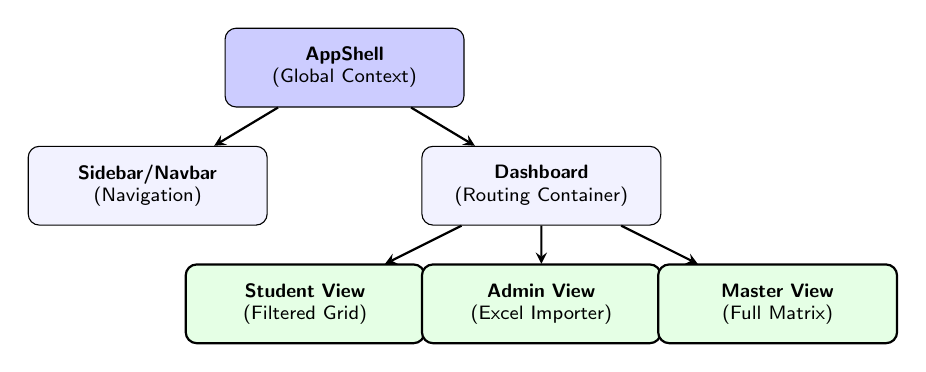
\begin{tikzpicture}[
    level 1/.style={sibling distance=5cm, level distance=1.5cm},
    level 2/.style={sibling distance=3cm, level distance=1.5cm},
    every node/.style={rectangle, draw, rounded corners, fill=blue!5, text width=2.8cm, align=center, font=\sffamily\scriptsize, minimum height=1cm},
    edge from parent/.style={draw, thick, ->, >=stealth}
]

\node[fill=blue!20] {\textbf{AppShell}\\(Global Context)}
    child {node {\textbf{Sidebar/Navbar}\\(Navigation)}}
    child {node {\textbf{Dashboard}\\(Routing Container)}
        child {node[fill=green!10] {\textbf{Student View}\\(Filtered Grid)}}
        child {node[fill=green!10] {\textbf{Admin View}\\(Excel Importer)}}
        child {node[fill=green!10] {\textbf{Master View}\\(Full Matrix)}}
    };
\end{tikzpicture}
\caption{Hierarchical Structure of the Core React Components}
\label{fig:component_tree}
\end{figure}

%-----------------------------------
\section{Role-Based Viewer Implementations}

The system provides several specialized views tailored to different stakeholders, summarized in Table~\ref{tab:view_mapping}.

\begin{table}[htbp]
\centering
\caption{Role-Based Component Mapping and Data Scope}
\label{tab:view_mapping}
\renewcommand{\arraystretch}{1.4}
\begin{tabularx}{\textwidth}{@{} l X l @{}}
\toprule
\textbf{Stakeholder Role} & \textbf{Component View} & \textbf{Primary Filter Parameter} \\
\midrule
Student & \texttt{TimetableViewer} & Semester \& Specific Section \\
Professor & \texttt{ProfessorTimetableViewer} & Faculty Email/ID \\
Department Admin & \texttt{RoomTimetableViewer} & Specific Room Name \\
Campus Admin & \texttt{MasterRoomViewer} & Building prefix (e.g., ``CC-3'', ``LT'') \\
Facility Staff & \texttt{FreeRoomViewer} & Temporal Matrix (Empty Rooms) \\
\bottomrule
\end{tabularx}
\end{table}

\subsection{Student Cohort View}
Given the complexity of modern curricula featuring numerous electives and minor tracks, a master timetable can be overwhelming. The \texttt{TimetableViewer} allows users to filter the master schedule by selecting a specific semester and section.

Crucially, it implements a \textbf{Smart Merging algorithm}. Often, core lectures are held for "All Sections" simultaneously, while practical laboratory sessions are split by specific section (e.g., "Sec A"). The merging algorithm intelligently filters the master data, pulling in slots explicitly assigned to the selected section \textit{and} slots assigned to the generic "All" section (WMC), combining them into a single, cohesive cohort schedule.

\subsection{Master Occupancy Viewer}
For campus administrators, the `MasterRoomViewer` provides a macro-level perspective. It displays a dense grid where rows represent physical rooms rather than student groups. Because an institution may have hundreds of rooms, this view implements a building-level filter. The system extracts the building prefix from the room name (e.g., identifying ``CC-3'' from ``CC-3-5106'') and allows the administrator to filter the grid, rendering a manageable overview of specific campus zones.

%-----------------------------------
\section{Export Mechanisms and Results}

To bridge the gap between the digital system and offline requirements, the platform implements robust export mechanisms.

\subsection{Client-Side PDF Generation}
Users can generate PDFs of their current view. This relies on the `html-to-image` library to capture the DOM state as a PNG, which is then embedded into a `jsPDF` document. A significant technical hurdle overcome during implementation was the handling of sticky CSS headers; the capture logic temporarily disables `position: sticky` properties on the DOM elements right before capture to ensure the entire scrollable area is rendered to the image buffer accurately.

\subsection{Google Sheets API Export}
The `RoomTimetableViewer` and `FreeRoomViewer` support bulk export directly to Google Sheets. Using the Google Identity Services client, the React application constructs a multi-layered batch update request. This request not only writes the raw string data into the cells but explicitly formats the workbookΓÇöcreating separate worksheets for different rooms, freezing header rows, applying pink and gray background colors to headers, and drawing solid bordersΓÇöresulting in a highly professional, ready-to-share document directly in the administrator's Google Drive.

\subsection{User Interface Evaluation}
The resulting application is a highly responsive, modern interface. By utilizing Tailwind CSS, the application maintains a clean, minimalist aesthetic with clear color coding (e.g., orange for practicals, green for tutorials). The elimination of page reloads between views, combined with the instantaneous clash detection, represents a monumental upgrade in usability and efficiency compared to traditional spreadsheet workflows.

%-----------------------------------
%-----------------------------------
%  NEW SECTIONS: SOLVER, EDITOR, GENERATOR
%-----------------------------------
%-----------------------------------



%-----------------------------------
\section{The Interactive Timetable Editor}
\label{sec:editor}

The \texttt{EditorView} component is where human judgment meets algorithmic output. It gives administrators an interactive, drag-and-drop interface for refining timetables---whether those timetables were generated by the solver or imported from Excel.

\subsection{Drag-and-Drop Slot Rearrangement}

The editor renders a dense 5-day $\times$ $N$-slot grid, where each scheduled session appears as a draggable card. Administrators can drag any session card from one cell to another to reassign its day and start time. The system automatically recalculates the end time based on the session's duration and validates that the new position does not fall in a lunch or break slot. All drag operations push the previous state onto a 30-level undo stack.

\subsection{Inline Editing}

Each session card exposes a hover-activated edit panel that allows inline modification of:
\begin{itemize}
    \item \textbf{Room Assignment:} A cascading two-step selector where the administrator first selects the room type (Lecture or Lab), then picks from filtered rooms of that type.
    \item \textbf{Professor Assignment:} A dropdown populated from the full professor list.
\end{itemize}

\subsection{Real-Time Conflict Visualization}

The editor implements a client-side clash detection algorithm that runs on every state change. Sessions involved in any conflict are highlighted with a red background and ring border. The algorithm checks the same constraints as the solver: room overlaps, professor overlaps, section overlaps (with elective exemptions), WMC-section conflicts, cross-basket elective clashes, and the 2+1 same-day lecture rule.

\subsection{Feasibility Check}

A dedicated ``Check Feasibility'' button constructs a full \texttt{SolverInput} from the current editor state, converts the slot positions into a \texttt{Solution} (Gene array), appends locked sessions from all other published timetables, and invokes the solver's \texttt{evaluate()} function. The result displays the total fitness score and the per-constraint violation breakdown, giving the administrator a precise understanding of remaining issues.

\subsection{LNS Auto-Fix}

When conflicts exist, the administrator can invoke the \textbf{Large Neighbourhood Search (LNS)} auto-fix~\cite{shaw1998using}. This routine:
\begin{enumerate}
    \item Identifies all session indices involved in any hard constraint violation (the ``clashing set'').
    \item Iterates for up to 1500 attempts. In each attempt, a random session from the clashing set is selected and a random mutation (relocate, time shift, or room change) is applied.
    \item If the mutation reduces the total fitness, the improved solution is accepted and the clashing set is refreshed.
    \item The process terminates early if all hard violations reach zero.
\end{enumerate}

The LNS targets only the problematic sessions rather than reoptimizing the entire schedule, making it significantly faster than a full solver run while preserving the administrator's manual adjustments to non-conflicting sessions. Figure~\ref{fig:lns_activity} illustrates this destroy-and-repair process.

\begin{figure}[htbp]
\centering
\begin{tikzpicture}[
    node distance=1.1cm,
    start/.style={draw, circle, fill=black, minimum size=6pt, inner sep=0pt},
    stop/.style={draw, circle, fill=black, minimum size=6pt, inner sep=0pt, double, double distance=1.5pt},
    action/.style={draw, rectangle, fill=green!8, rounded corners=3pt, text width=5.5cm, align=center, font=\sffamily\scriptsize, minimum height=0.6cm},
    decision/.style={draw, diamond, aspect=2.5, fill=orange!10, text width=2cm, align=center, font=\sffamily\scriptsize, inner sep=1pt},
    arrow/.style={draw, thick, ->, >=stealth, font=\sffamily\tiny}
]

\node[start] (s) {};
\node[action, below=of s] (find) {Identify Clashing Set\\(all sessions with hard violations)};
\node[decision, below=of find] (empty) {Clashing set\\empty?};
\node[action, below=1.2cm of empty] (pick) {Pick random session from clashing set};
\node[action, below=of pick] (mut) {Apply random mutation\\(relocate / time shift / room swap)};
\node[action, below=of mut] (ev) {Evaluate candidate fitness};
\node[decision, below=of ev] (better) {Improved?};
\node[action, below left=1cm and 0cm of better] (acc) {Accept candidate\\Refresh clashing set};
\node[decision, below=2cm of better] (maxiter) {Max attempts\\reached?};
\node[stop, right=2cm of empty] (done1) {};
\node[stop, below=0.8cm of maxiter] (done2) {};

\draw[arrow] (s) -- (find);
\draw[arrow] (find) -- (empty);
\draw[arrow] (empty) -- node[right] {No} (pick);
\draw[arrow] (empty) -- node[above] {Yes (feasible)} (done1);
\draw[arrow] (pick) -- (mut);
\draw[arrow] (mut) -- (ev);
\draw[arrow] (ev) -- (better);
\draw[arrow] (better) -- node[left] {Yes} (acc);
\draw[arrow] (better.east) -- ++(1.5,0) node[above left, font=\sffamily\tiny] {No} |- (maxiter);
\draw[arrow] (acc) |- (maxiter);
\draw[arrow] (maxiter) -- node[right] {Yes} (done2);
\draw[arrow] (maxiter.west) -- ++(-2,0) node[above right, font=\sffamily\tiny] {No} |- (pick);

\end{tikzpicture}
\caption{Activity Diagram: LNS Destroy-and-Repair Auto-Fix}
\label{fig:lns_activity}
\end{figure}

